\documentclass{article}

% if you need to pass options to natbib, use, e.g.:
%     \PassOptionsToPackage{numbers, compress}{natbib}
% before loading neurips_2019

% ready for submission
% \usepackage{neurips_2019}

% to compile a preprint version, e.g., for submission to arXiv, add add the
% [preprint] option:
%     \usepackage[preprint]{neurips_2019}

% to compile a camera-ready version, add the [final] option, e.g.:
\usepackage[]{neurips_2019}

% to avoid loading the natbib package, add option nonatbib:
%     \usepackage[nonatbib]{neurips_2019}

\usepackage[utf8]{inputenc} % allow utf-8 input
\usepackage[T1]{fontenc}    % use 8-bit T1 fonts
\usepackage{hyperref}       % hyperlinks
\usepackage{url}            % simple URL typesetting
\usepackage{booktabs}       % professional-quality tables
\usepackage{amsfonts}       % blackboard math symbols
\usepackage{nicefrac}       % compact symbols for 1/2, etc.
\usepackage{microtype}      % microtypography

\usepackage[dvipsnames]{xcolor}
\usepackage[normalem]{ulem}
\usepackage{graphicx}
\usepackage{subfigure}
\newif{\ifhidecomments}


\title{Reproducibility report formatting instructions for ML Reproducibility Challenge 2021}

% The \author macro works with any number of authors. There are two commands
% used to separate the names and addresses of multiple authors: \And and \AND.
%
% Using \And between authors leaves it to LaTeX to determine where to break the
% lines. Using \AND forces a line break at that point. So, if LaTeX puts 3 of 4
% authors names on the first line, and the last on the second line, try using
% \AND instead of \And before the third author name.

\author{%
  Benyuan Wang \\
  Department of Systems Design Engineering\\
  University of Waterloo\\
  200 University Avenue West Waterloo, ON, Canada  N2L 3G1 \\
  \texttt{b376wang@uwaterloo.ca} \\
  % examples of more authors
  \And
  Dening Lu \\
  Department of Systems Design Engineering\\
  University of Waterloo\\
  200 University Avenue West Waterloo, ON, Canada  N2L 3G1 \\
  \texttt{d62lu@uwaterloo.ca} \\
  \AND
  Department of Systems Design Engineering\\
  University of Waterloo\\
  200 University Avenue West Waterloo, ON, Canada  N2L 3G1 \\
  \texttt{w57liang@uwaterloo.ca} \\
  % \And
  % Coauthor \\
  % Affiliation \\
  % Address \\
  % \texttt{email} \\
  % \And
  % Coauthor \\
  % Affiliation \\
  % Address \\
  % \texttt{email} \\
}

\begin{document}

\maketitle

\section*{\centering Reproducibility Summary}

\textit{Template and style guide to \href{https://paperswithcode.com/rc2021}{ML Reproducibility Challenge 2021}. The following section of Reproducibility Summary is \textbf{mandatory}. This summary \textbf{must fit} in the first page, no exception will be allowed. When submitting your report in OpenReview, copy the entire summary and paste it in the abstract input field, where the sections must be separated with a blank line.
}

\subsection*{Scope of Reproducibility}

We mainly reproduce the claim in the original paper that Swin Transformer achieves strong performance on the recognition task of image classification.

\subsection*{Methodology}

We used the code provided by the author on github, we used the Swin Transformer proposed by the author to reproduce the classification part of the experiment, and we used the Tesla P100 GPU provided by colab to complete our experiment. Since the data set used by the author is too large, we cannot upload it to Google Drive, so we used a smaller data set to complete our experiments. We have also completed many experiments beyond the original text.

\subsection*{Results}

We give the accuracy and loss graphs of the three variant structures in the original paper, and also give many of our results beyond the original paper, such as ablation experiments, hyperparameters comparison, Non-Local transformer, A-SCN transformer, Point-Attention transformer and Offset-Attention transformer.

\subsection*{What was easy}

The original paper provided a chart that included a description of the architecture and performance, which provided us with a clear benchmark to compare our results. In addition, all the experimental data set links and codes are also included in the paper itself.

\subsection*{What was difficult}

The biggest problem we face is the inability to achieve the same experimental conditions as the original paper author. The data set used by the author is too large for us to upload it to colab, so we can only use a smaller data set, and the generated data results cannot be compared with the original paper. And because our colab memory is small, we cannot set the batch size to 256 or greater, which also limits the reproduction of our paper.


\subsection*{Communication with original authors}

Briefly describe how much contact you had with the original authors (if any).
\newpage
\textit{\textbf{The following section formatting is \textbf{optional}, you can also define sections as you deem fit.
\\
Focus on what future researchers or practitioners would find useful for reproducing or building upon the paper you choose.}}
\section{Introduction}
The paper we selected is “Swin Transformer: Hierarchical Vision Transformer using Shifted Windows”, which has been published in CVPR2021. This paper proposes a novel image processing method based on the transformer mechanism which has achieved significant progress in natural language processing (NLP). Swin Transformer aims to develop an efficient backbone network for image processing such as classification, object detection and segmentation. To reduce the computational complexity, Swin Transformer proposes a window-based transformer algorithm, i.e., applying the transformer method to fixed-size windows instead of the global image scale. And to build connections with different non-overlapping windows, Swin Transformer introduces shifted window module. Because of the hierarchical design and cross-window connection, Swin Transformer, as a backbone network, surpasses the previous state-of-the-art method in terms of image classification, object detection and segmentation. 
\section{Scope of reproducibility}

Swin Transformer has made two improvements compared to the previous ViT:

(1)Introduce a commonly used hierarchical construction method in CNN to construct a hierarchical Transformer.

(2)Introduce the idea of locality, and perform self-attention calculation in the window area without overlap.

The authors make one key claim:
\begin{itemize}
\item Claim 

The proposed Swin Transformer achieves strong performance on the recognition task of image classification.

\end{itemize}


%\jdcomment{To organizers: I asked my students to connect the main claims and the experiments that supported them. For example, in this list above they could have ``Claim 1, which is supported by Experiment 1 in Figure 1.'' The benefit was that this caused the students to think about what their experiments were showing (as opposed to blindly rerunning each experiment and not considering how it fit into the overall story), but honestly it seemed hard for the students to understand what I was asking for.}

\section{Methodology}

We used the code provided by the author on github, we used the Swin Transformer proposed by the author to reproduce the classification part of the experiment, and we used the Tesla P100 GPU provided by colab to complete our experiment. Since the data set used by the author is too large, we cannot upload it to Google Drive, so we used a smaller data set to complete our experiments. We have also completed many experiments beyond the original text, such as ablation experiments, hyperparameters comparison, Non-Local transformer, A-SCN transformer, Point-Attention transformer and Offset-Attention transformer.

\subsection{Model descriptions}

Swin Transformer has made two improvements

(1)Introduce a commonly used hierarchical construction method in CNN to construct a hierarchical Transformer.

\begin{figure}[h]
\centering
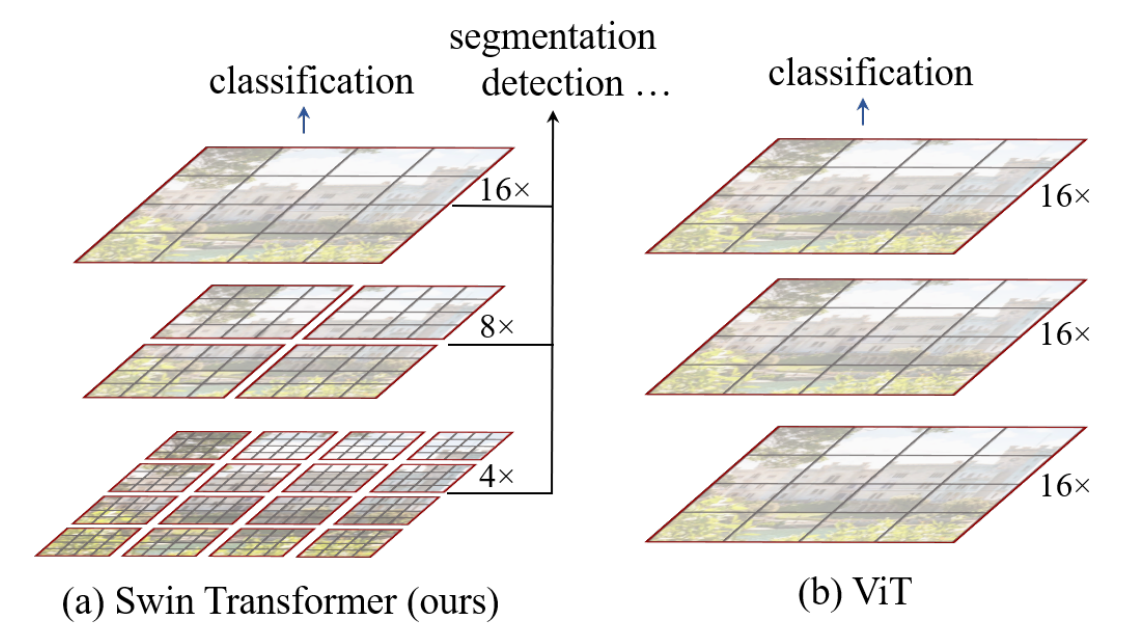
\includegraphics[scale=0.5]{1}
\caption{(a) The proposed Swin Transformer builds hierarchical
feature maps by merging image patches (shown in gray) in deeper layers and has linear computation complexity to input image size due to computation of self-attention only within each local window (shown in red).
(b) In contrast, previous vision Transformers produce feature maps of a single low resolution and have quadratic computation complexity to input image size due to computation of self-attention globally.}
\label{fig:1}
\end{figure}

(2)Introduce the idea of locality, and perform self-attention calculation in the window area without overlap.
\begin{figure}[h]
\centering
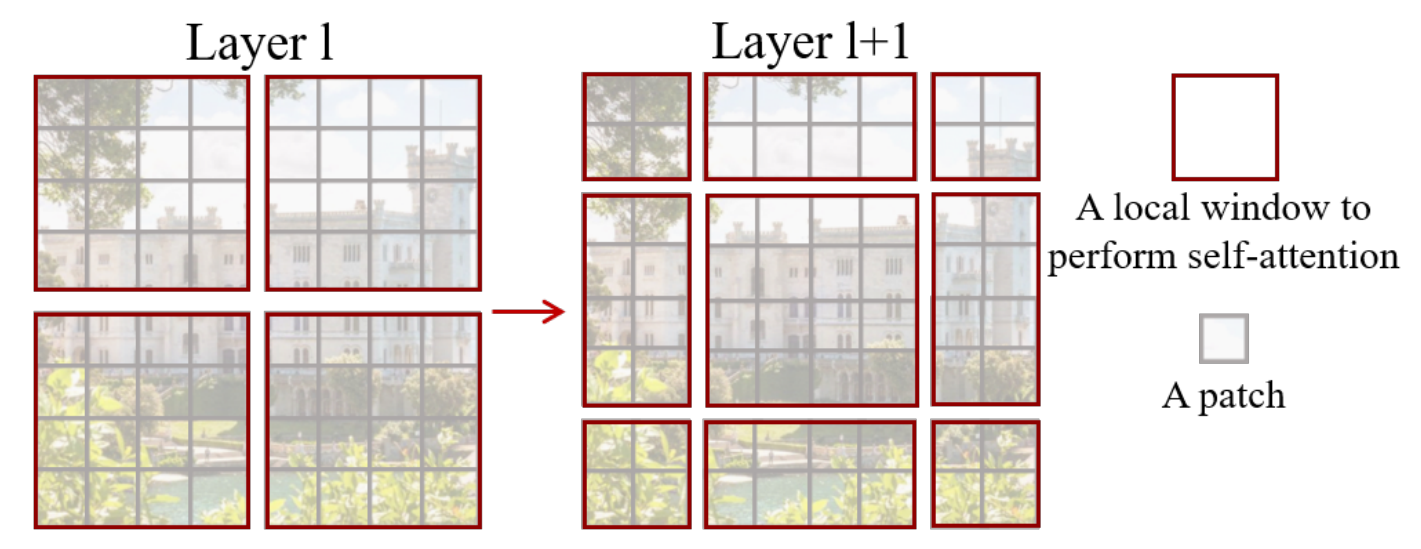
\includegraphics[scale=0.5]{2}
\caption{An illustration of the shifted window approach for computing self-attention in the proposed Swin Transformer architecture. In layer l (left), a regular window partitioning scheme is adopted, and self-attention is computed within each window. In the next layer l + 1 (right), the window partitioning is shifted, resulting in new windows. The self-attention computation in the new windows crosses the boundaries of the previous windows in layer l, providing connections among them.}
\label{fig:2}
\end{figure}

The red area is the local window and the gray area is the patch. W-MSA divides the input image into windows that do not overlap, and then performs self-attention calculations in different windows. Assuming that a picture has h x w patches, and each window contains M x M patches, the computational complexity of MSA and W-MSA are:
$$\Omega(MSA) = 4hwC^2+2(hw)^2C$$
$$\Omega(W-MSA) = 4hwC^2+2M^2hwC$$
Since the number of window patches is much smaller than the number of image patches, the computational complexity of W-MSA has a linear relationship with the image size.
In addition, although W-MSA reduces the computational complexity, there is a lack of information exchange between windows that do not overlap, so the authors further introduce shifted window partition to solve the information exchange problem of different windows, and use W-MSA and SW-MSA alternately in two consecutive Swin Transformer Blocks. 

\begin{figure}[h]
\centering
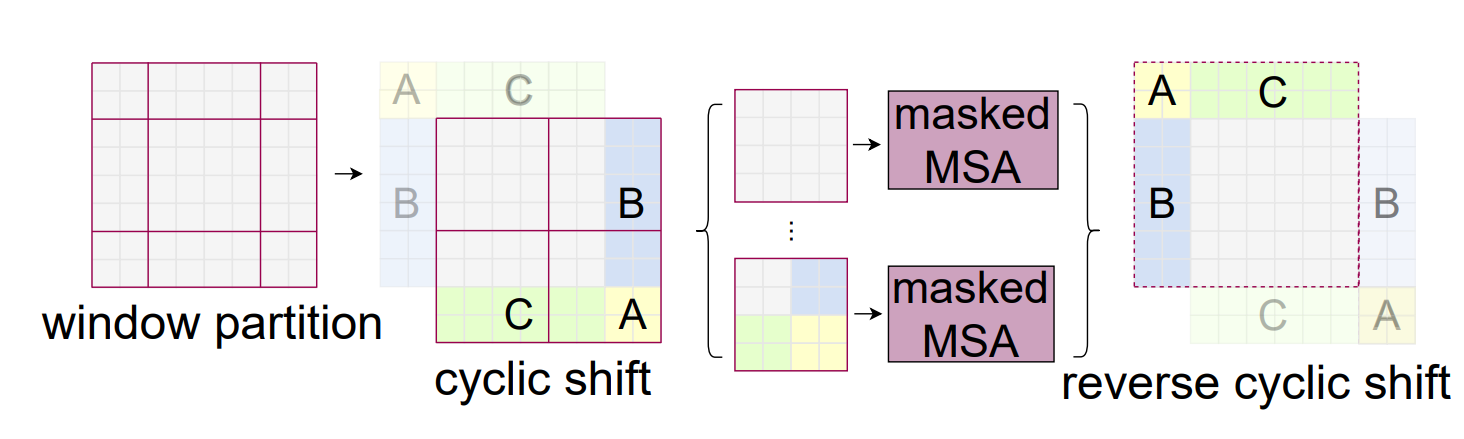
\includegraphics[scale=0.6]{3}
\caption{Illustration of an efficient batch computation approach
for self-attention in shifted window partitioning.}
\label{fig:3}
\end{figure}

(3)frame

\begin{figure}[h]
\centering
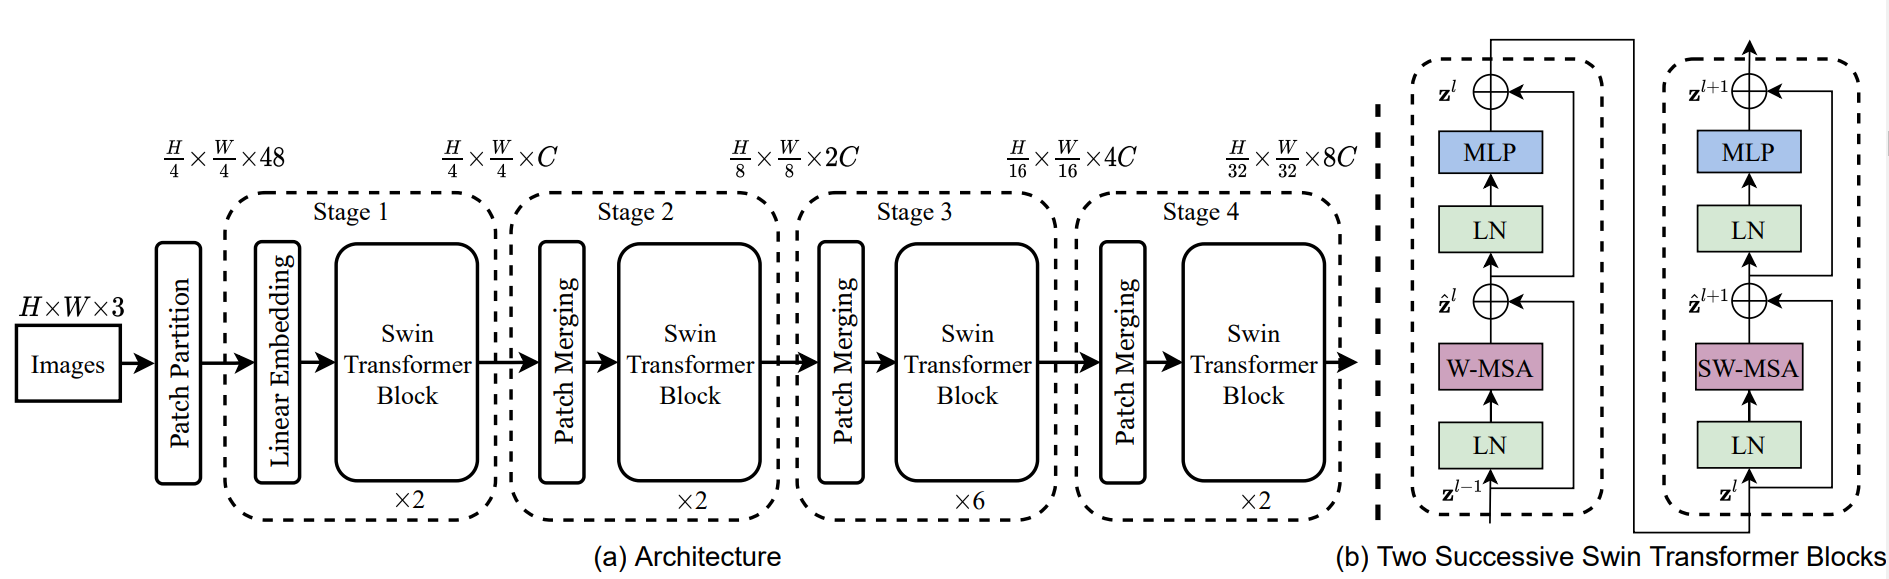
\includegraphics[scale=0.5]{4}
\caption{(a) The architecture of a Swin Transformer (Swin-T); (b) two successive Swin Transformer Blocks. W-MSA and SW-MSA are multi-head self attention modules with regular and shifted windowing configurations, respectively.}
\label{fig:4}
\end{figure}

The input picture with the shape H x W x 3 is divided into non-overlapping patch through patch partition, where each patch has a size of 4x4, then the feature dimension of each patch is 4x4x3=48, and the number of patch blocks is H/4 x W/4. At the first stage, use a linear embedding to change the dimension of the patch feature to C, and then send it to the Swin Transformer Block. Stage 2 to 4 are similar to the stage 1. 
\newpage
\subsection{Datasets}

Since the data set used in the author’s experiment is too large, we have no conditions to use the same data set as the author, so we use a smaller data set, where the training set contains 15 categories and a total of 1500 grayscale images, and the test set contains 15 categories and a total of 2985 grayscale images.

\subsection{Hyperparameters}

We build our base model, called Swin-B, to have the similar model size and computation complexity to ViTB/DeiT-B. We also introduce Swin-T and Swin-S, which are versions of about 0.25× and 0.5× the model size and computational complexity, respectively. Note that the complexity of Swin-T and Swin-S are similar to those of ResNet-50 (DeiT-S) and ResNet-101, respectively. The window size is set to M = 7 by default. The query dimension of each head is d = 32, and the expansion layer of each MLP is $\alpha = 4$, for all experiments. The architecture hyper-parameters of these model variants are:
\begin{itemize}
\item Swin-T:C = 96,layernumbers={2,2,6,2},batch size=128,learning rate = 5e-4

\item Swin-S:C = 96,layernumbers={2,2,18,2},batch size=64,learning rate = 5e-4

\item Swin-B:C = 128,layernumbers={2,2,18,2},batch size=64,learning rate = 5e-4

\end{itemize}
where C is the channel number of the hidden layers in the
first stage.
\newpage
\subsection{Experimental setup and code}

The code for our experiment has been uploaded, and the entire experiment was run using the Tesla-P100 GPU provided by colab.

\subsection{Computational requirements}

The entire experiment was run using the Tesla-P100 GPU provided by colab.You can view our GPU information from the picture in the appendices.

The time consumed for each experiment is as follows:

\begin{itemize}
\item Reproduction experiment in the original text with pretrained model, Swin-T:2:56:15, Swin-S:4:00:08, Swin-B:5:57:48

\item Ablation experiment based on Swin-B with pretrained model, Remove position embedding:3:02:11, Remove shifted window:2:57:26, Remove residual:2:59:27, Remove dropout:3:12:27


\item Improve the module of self-attention with pretrained model, Non-Local: 2:52:17, A-SCN: 2:08:39, Point-Attention: 2:10:18, Offset-Attention: 3:00:10


\item Improve the module of self-attention without pretrained model, Non-Local: 3:12:00, A-SCN: 2:27:38, Point-Attention: 2:28:52, Offset-Attention: 3:17:41

\end{itemize}


\section{Results}
\label{sec:results}
Our results support the claims in the original text, and swin transformer does effectively improve the accuracy of image classification.

\subsection{Results reproducing original paper}

We mainly reproduce the accuracy of image classification of the three variants proposed in the article, which proves that swin transformer achieves good performance.

\subsubsection{Result}
In this part, we give the accuracy and loss diagrams of three different structures Swin-B,Swin-T and Swin-S. Our three structures all use the pre-trained model provided by the author.



    \begin{table}[h]
		\centering
		\begin{tabular}{|c|c|c|c|c|}\hline
			Backbone&image size&acc@1&acc@5&Training time\\
\hline
			Swin-T&224*224&95.310&99.899&2:56:15\\
			Swin-S&224*224&95.444&99.765&4:00:08\\
			Swin-B&224*224&95.946&99.899&5:57:48\\
\hline
		\end{tabular}
		\caption{Comparison of different backbones.}
		\label{tab:1}
	\end{table}

\begin{figure}[htbp]
\centering
\subfigure[Swin-B]{
\begin{minipage}[t]{0.33\linewidth}
\centering
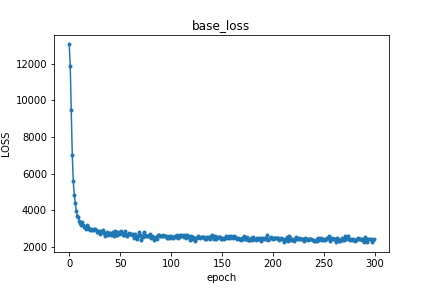
\includegraphics[scale=0.35]{base_loss}
%\caption{fig1}
\end{minipage}%
}%
\subfigure[Swin-T]{
\begin{minipage}[t]{0.33\linewidth}
\centering
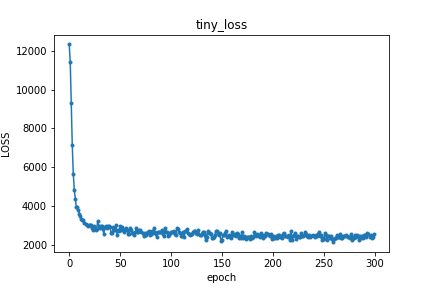
\includegraphics[scale=0.35]{tiny_loss}
%\caption{fig2}
\end{minipage}%
}%
\subfigure[Swin-S]{
\begin{minipage}[t]{0.33\linewidth}
\centering
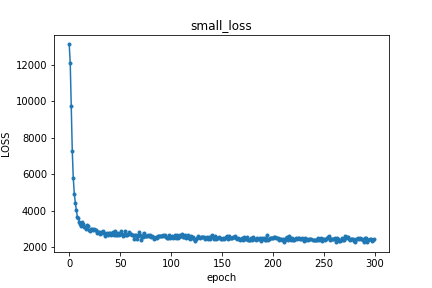
\includegraphics[scale=0.35]{small_loss}
%\caption{fig2}
\end{minipage}
}%
\centering
\caption{Loss graph of three structures.}
\end{figure}


\subsection{Results beyond original paper}

In the part beyond the original paper, we mainly completed the ablation experiment, hyperparameter comparison and improve the module of self-attention.

\subsubsection{Ablation experiment}

In this part, we performed ablation experiments based on Swin-T, and removed position embedding, shifted window, residual and dropout respectively. Then we showed the accuracy and loss graphs of each experiment.

\begin{figure}[htbp]
\centering
\subfigure[Remove position embedding]{
\begin{minipage}[t]{0.25\linewidth}
\centering
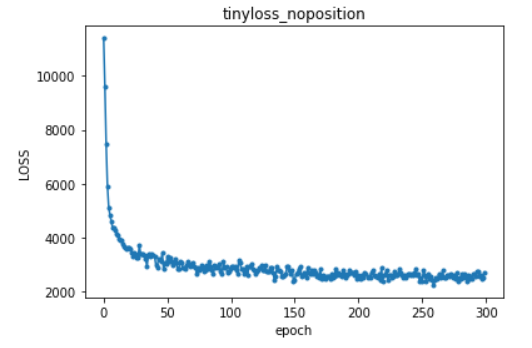
\includegraphics[scale=0.45]{no1}
%\caption{fig1}
\end{minipage}%
}%
\subfigure[Remove shifted window]{
\begin{minipage}[t]{0.25\linewidth}
\centering
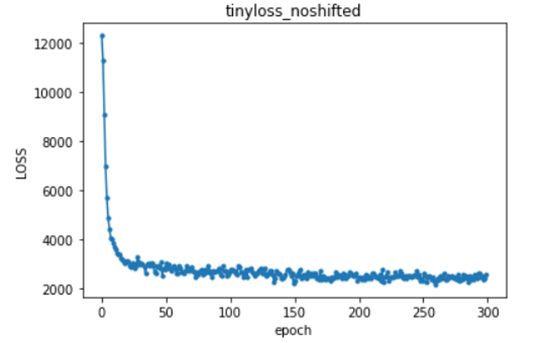
\includegraphics[scale=0.45]{no2}
%\caption{fig2}
\end{minipage}%
}%
\subfigure[Remove residual]{
\begin{minipage}[t]{0.25\linewidth}
\centering
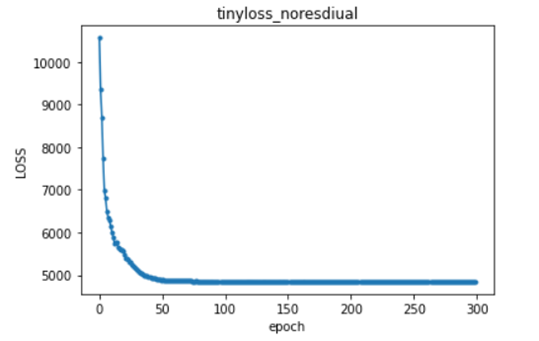
\includegraphics[scale=0.45]{no3}
%\caption{fig3}
\end{minipage}
}%
\subfigure[Remove dropout]{
\begin{minipage}[t]{0.25\linewidth}
\centering
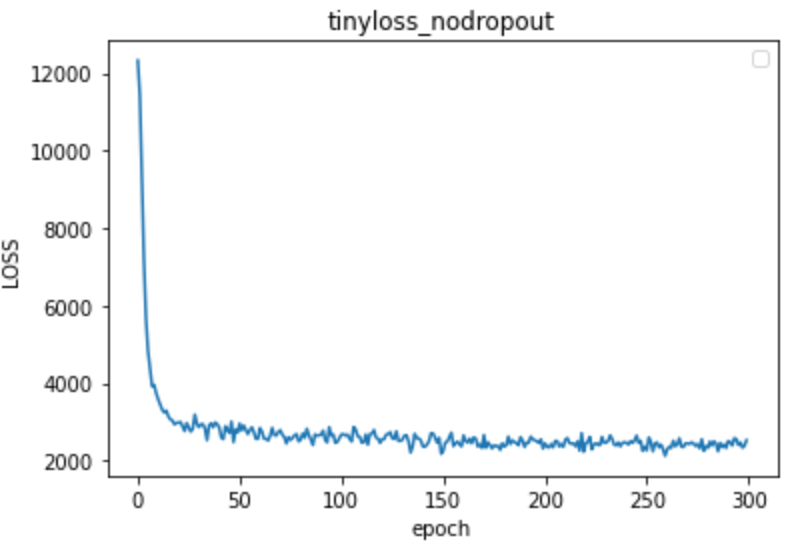
\includegraphics[scale=0.28]{no4}
%\caption{fig4}
\end{minipage}
}%
\centering
\caption{Loss graph of Ablation experiment.}
\end{figure}

\begin{table}[h]
		\centering
		\begin{tabular}{|c|c|c|c|c|}\hline
			Ablation method&image size&acc@1&acc@5&Training time\\
\hline
			Remove position embedding&224*224&93.936&99.866&3:02:11\\
			Remove shifted window&224*224&94.807&99.966&2:57:26\\
			Remove residual&224*224&4.121&26.600&2:59:27\\
			Remove dropout&224*224&95.510&99.966&3:12:27\\
\hline
		\end{tabular}
		\caption{Results of ablation experiments.}
		\label{tab:2}
\end{table}

\subsubsection{Hyperparameter comparison}

In this part, we made a hyperparameter comparison based on Swin-T, and tested learning rates of 1e-3, 5e-3, and 1e-4, and batch sizes of 16, 32, and 64. Then we showed the accuracy and loss graphs of each experiment.


\begin{figure}[htbp]
\centering
\subfigure[Learning rate comparison.]{
\begin{minipage}[t]{0.5\linewidth}
\centering
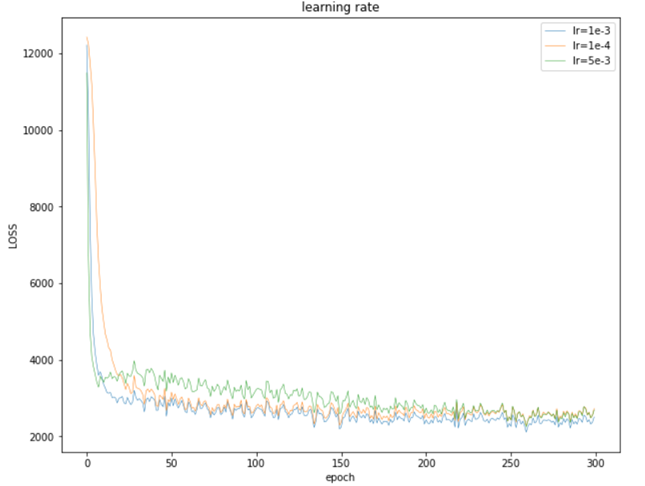
\includegraphics[scale=0.7]{7}
%\caption{fig1}
\end{minipage}%
}%
\subfigure[Batch size comparison.]{
\begin{minipage}[t]{0.5\linewidth}
\centering
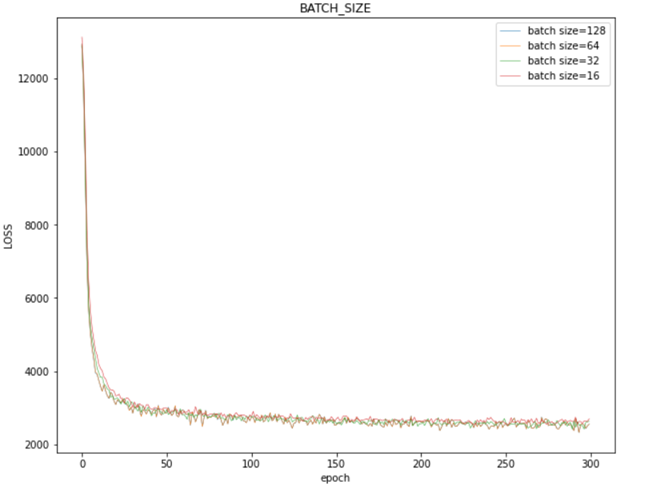
\includegraphics[scale=0.7]{8}
%\caption{fig2}
\end{minipage}%
}%
\centering
\caption{Loss graph of Hyperparameter comparison.}
\end{figure}


    \begin{table}[h]
		\centering
		\begin{tabular}{|c|c|c|c|c|}\hline
			Learning rate&image size&acc@1&acc@5&Training time\\
\hline
			1e-3&224*224&94.874&99.899&2:27:10\\
			5e-3&224*224&94.405&99.832&2:27:30\\
			1e-4&224*224&95.645&99.933&2:27:31\\
\hline
			Batch size&image size&acc@1&acc@5&Training time\\
\hline
			16&224*224&95.678&99.966&3:10:10\\
			32&224*224&95.779&99.933&2:56:35\\
			64&224*224&95.310&99.899&2:56:15\\
\hline

\hline
		\end{tabular}
		\caption{Results of hyperparameter comparison experiments.}
		\label{tab:3}
	\end{table}



\newpage
\subsubsection{Improve the module of self-attention }

In this section, we utilize some self attention variants to try to improve the network. The first one is the self-attention mechanism used in swin transformer. And the other five variants are proposed in different published papers. From my perspective, all these variants focus on doing some operation between the input and output, which are similar with residual architecture.

    \begin{table}[h]
		\centering
		\begin{tabular}{|c|c|c|c|c|}\hline
			Transformer with pretrained model.&image size&acc@1&acc@5&Training time\\
\hline
			Swin transformer&224*224&95.310&99.899&2:56:15\\
			Non-Local[3]&224*224&83.48&99.531&2:52:17\\
			A-SCN[4]&224*224&66.33&99.219&2:08:39\\
			Point-Attention[5]&224*224&86.23&99.645&2:10:18\\
			Offset-Attention[6]&224*224&90.89&99.926&3:00:10\\
\hline
			Transformer without pretrained model.&image size&acc@1&acc@5&Training time\\
\hline
			Swin transformer&224*224&76.35&98.438&2:56:20\\
			Non-Local[3]&224*224&76.88&99.219&3:12:00\\
			A-SCN[4]&224*224&52.80&94.531&2:27:38\\
			Point-Attention[5]&224*224&75.58&98.438&2:28:52\\
			Offset-Attention[6]&224*224&75.01&98.559&3:17:41\\
\hline
		\end{tabular}
		\caption{Results of some self attention variants.}
		\label{tab:4}
	\end{table}




\section{Discussion}


\begin{itemize}
\item For the swin transformer proposed in the original paper, we found that its classification performance is indeed significantly improved over the previous method.And as the computational complexity increases, we can find that the accuracy is slightly improved. In our previous work, using the VGG network to classify the same data set can only achieve an accuracy of about 90\%[2] , While using the Swin-T model in the original text can achieve an accuracy of 95\%.

\item Ablation one

We remove the position embedding module. For the transformer in 2D image processing, It is important to add position information to transformer. Without the position embedding, transformer mechanism may not distinguish two images when you swap different areas of the image, which may reduce the performance of the method. And the classification accuracy of the method without position embedding also confirm this. The accuracy is lower than method with position information.

\item Ablation two

We remove the shifted window module. From the paper, we can see that the authors utilize the local transformer in a hierarchical manner, and to establish the connection between different windows, shifted window module is designed. So, without shifted window, different windows may not connect each other, and it may result in the loss of information. So from the ablation results, the method without shifted window get a relatively lower classification accuracy.

\item Ablation three

We remove the residual architecture, which is like a skip connection. Residual architecture can be simply considered as adding the output of the module to the input of the module, which can prevent the vanishing gradient problem of the deep network effectively, and prevent the loss of information. 
So when we remove this architecture, the accuracy drops so sharply, which really shocked me. We did realize that the accuracy would drop without residual, but the decline exceeded my expectations. And We repeated this experiment for several times, the results are similar. So the residual architecture did play an important role in the deep learning network.

\item Ablation four

We remove the dropout module, in other words, we set the dropout rate to zero.
What the dropout does is to reduce the degree of overfitting for the network, and the bachnormalization has the similar effect on the network. 
This operation can improve the generalization performance of the network, because after disabling some perceptrons, the network will not rely too much on some local features.
But on the other hand, dropout also means lose some information, so it may have a little bad influence on accuracy. In this case, we use pretrained model which is generated from ImageNet10K dataset. And train our own small dataset, it is like a fine tuning, so removing dropout can help to save more feature information, which maybe a reason for the increase in accuracy.

\item Hyperparameter comparison

We modified the batch size to 64, 32 and 16 respectively under the model based on Swin-T. The batch size slightly affects the convergence process of loss. The larger the batch size, the faster the convergence, but the accuracy is slightly lower. However, in our experiment, the effect of modifying the batch size on the accuracy is not obvious, which may be due to the small data set we chose.
We modify the learning rates respectively to 1e-3, 5e-3 and 1e-4 based on the Swin-T model. As an important hyperparameter in supervised learning and deep learning, learning rate determines whether the objective function can converge to a local minimum and when it converges to the minimum. A proper learning rate can make the objective function converge to a local minimum in a proper time. When the learning rate is set too small, the convergence process will become very slow. When the learning rate is set too large, the gradient may oscillate around the minimum value, and may even fail to converge. In our experiments, we found that when we set the learning rate to 1e-4, we can achieve the best accuracy.

\item Improve the module of self-attention

In this section, I utilize some self attention variants to try to improve the network. The first one is the self-attention mechanism used in swin transformer. And the other five variants are proposed in different published papers. From my perspective, all these variants focus on doing some operation between the input and output, which are similar with residual architecture. 
In the case of using pretrained model, since this pretrained model is generated from the network with the first self attention variant, so it is reasonable that the network with the first variant achieves the best result. So we think this experiment is a little unfair.
In the case of training the network from scratch, non local variant gets the highest classification accuracy, which prove that we can replace the original self attention mechanism with non local variant, to improve the performance of the network. And in terms of the running time, point attention variant achieve the similar accuracy with swin transformer, but the training time is much less than the latter, so this also maybe an increase in efficiency.
\end{itemize}

\subsection{What was easy}
The biggest problem we face is the inability to achieve the same experimental conditions as the original paper author. The data set used by the author is too large for us to upload it to colab, so we can only use a smaller data set, and the generated data results cannot be compared with the original paper. And because our colab memory is small, we cannot set the batch size to 256 or greater, which also limits the reproduction of our paper. The code is simple and easy to read, the environment configuration is relatively simple, and the paper is relatively simple to follow.

\subsection{What was difficult}

The biggest problem we face is the inability to achieve the same experimental conditions as the original paper author. The data set used by the author is too large for us to upload it to colab, so we can only use a smaller data set, and the generated data results cannot be compared with the original paper. And because our colab memory is small, we cannot set the batch size to 256 or greater, which also limits the reproduction of our paper.

\section*{References}
[1] Ze Liu, Yutong Lin, Yue Cao, Han Hu, Yixuan Wei, Zheng Zhang, Stephen Lin, Baining Guo. Swin Transformer: Hierarchical Vision Transformer using Shifted Windows. arXiv:2103.14030 [cs.CV]

[2] Karen Simonyan, Andrew Zisserman.Very Deep Convolutional Networks for Large-Scale Image Recognition. arXiv:1409.1556 [cs.CV]

[3] Xiaolong Wang, Ross Girshick, Abhinav Gupta, and Kaiming He. Non-local neural networks. In Proceedings of the IEEE Conference on Computer Vision and Pattern Recognition, pages 7794–7803, 2018.

[4] Saining Xie, Sainan Liu, Zeyu Chen, and Zhuowen Tu. Attentional shapecontextnet for point cloud recognition. In Proceedings of the IEEE Conference on Computer Vision and Pattern Recognition, pages 4606–4615, 2018. 

[5] Mingtao Feng, Liang Zhang, Xuefei Lin, Syed Zulqarnain Gilani, and Ajmal Mian. Point attention network for semantic segmentation of 3d point clouds. Pattern Recognition, 107:107446, 2020.

[6] Meng-Hao Guo, Jun-Xiong Cai, Zheng-Ning Liu, Tai-Jiang
Mu, Ralph R Martin, and Shi-Min Hu. Pct: Point cloud transformer. Computational Visual Media, 7:pages187–199, 2021.

\section*{Appendices}

The three of us studied this paper together. Weidong Liang is responsible for running the three variants provided in the original paper and the learning rate part of the hyperparameter comparison experiment. Dening Lu is responsible for running the batch size part of the hyperparameter comparison experiment, the ablation experiment and the Improve the module of self-attention part. Benyuan Wang is responsible for writing the report. In the production of ppt, Weidong Liang is responsible for the theoretical explanation part, Benyuan Wang is responsible for the original text experiment reproduction and hyperparameter comparison part, and Dening Lu is responsible for the ablation experiment and the Improve the module of self-attention part.

\begin{figure}[h]
\centering
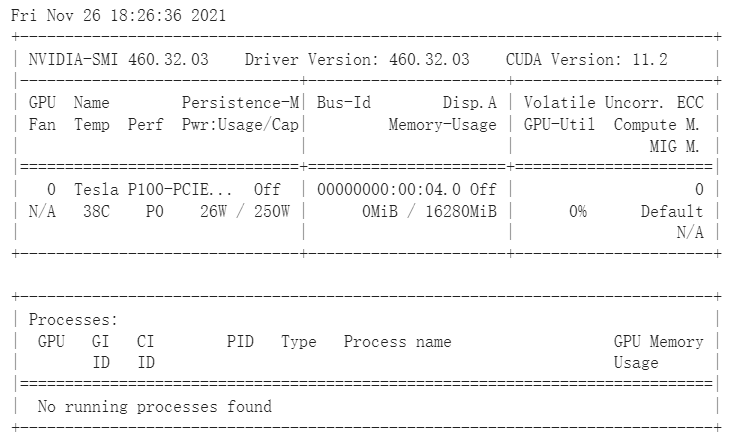
\includegraphics[scale=0.7]{5}
\caption{GPU information}
\label{fig:5}
\end{figure}

\end{document}
